\documentclass[aspectratio=169,xcolor=dvipsnames, t]{beamer}
\usepackage{fontspec} % Allows using custom font. MUST be before loading the theme!
\usetheme{SimplePlusAIC}
\usepackage{hyperref}
\usepackage{graphicx} % Allows including images
\usepackage{booktabs} % Allows the use of \toprule, \midrule and  \bottomrule in tables
\usepackage{svg} %allows using svg figures
\usepackage{tikz}
\usepackage{makecell}
\usepackage{wrapfig}
\usepackage[czech]{babel}
\usepackage{tabularx}
\newcommand{\R}{\mathbb{R}}
\newcommand{\N}{\mathbb{N}}


\title[]{Internet} % The short title appears at the bottom of every slide, the full title is only on the title page
\subtitle{}

\author[Dusart]{Eric Dusart}
\institute[GEVO]{Gymnázium Evolution Jižní Město}
\date{\today}


\begin{document}

\maketitlepage
{
\setbeamertemplate{background}
{
    
\includegraphics[width=\paperwidth,height=\paperheight]{AICStyleData/logos/mene_polygonu_bg.png}
}
\begin{frame}[t]{Obsah}
    \tableofcontents
\end{frame}
}


\section{Historie}
\setbeamertemplate{background}
{
    
\includegraphics[width=\paperwidth,height=\paperheight]{AICStyleData/logos/mene_polygonu_bg.png}
}
\begin{frame}{Historie}
    \vspace{-0.5cm}
    \begin{columns}
    \begin{column}{0.45\textwidth}
    \begin{itemize}
        \item Internet je propojení počítačů celým světem pomocí počítačových sítí. 
        \item Komunikují mezi sebou pomocí rodiny protokolů TCP/IP.
        \item Služby fungující pomocí internetu $\rightarrow$ webové stránky, sociální sítě, chaty, videohovory, e-mail, \ldots
        \item Roku 1969 byla zprovozněna jedna z prvních sítí ARPANET se čtyřmi uzly (USA).
    \end{itemize}
\end{column}
\begin{column}{0.45\textwidth}
    \begin{figure}
        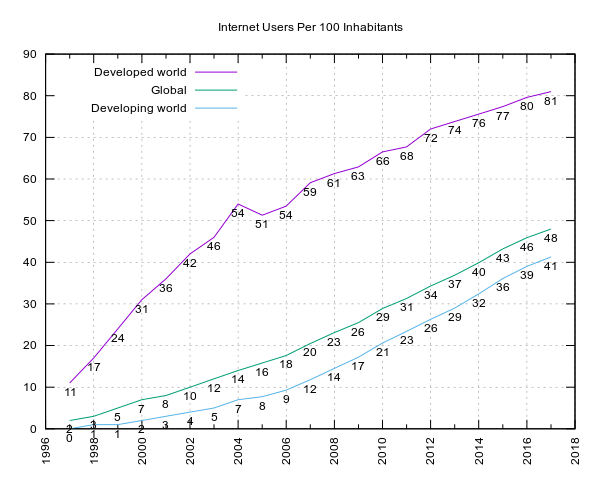
\includegraphics[width=\textwidth]{Internet_users_per_100_inhabitants_ITU}
        \caption{Počet internetových uživatelů na 100 obyvatel.}
    \end{figure}
\end{column}
\end{columns}
\end{frame}

\section{Internetové služby}
\subsection{Světová široká pavučina}
\setbeamertemplate{background}
{
    
\includegraphics[width=\paperwidth,height=\paperheight]{AICStyleData/logos/mene_polygonu_bg.png}
}
\begin{frame}{Internetové služby: World wide web}
    \vspace{-0.5cm}
    \begin{columns}
    \begin{column}{0.45\textwidth}
        \begin{itemize}
            \item Systém webových stránek zobrazovaných pomocí webového prohlížeče
            \item Používají protokoly HTTP, nebo HTTPS.
            \item Koncem roku 1990 Tim Berners-Lee, zakladatel WWW, spustil první webový server na světě: \href{https://info.cern.ch/}{info.cern.ch}
        \end{itemize}
\end{column}
\begin{column}{0.45\textwidth}
    \begin{figure}
        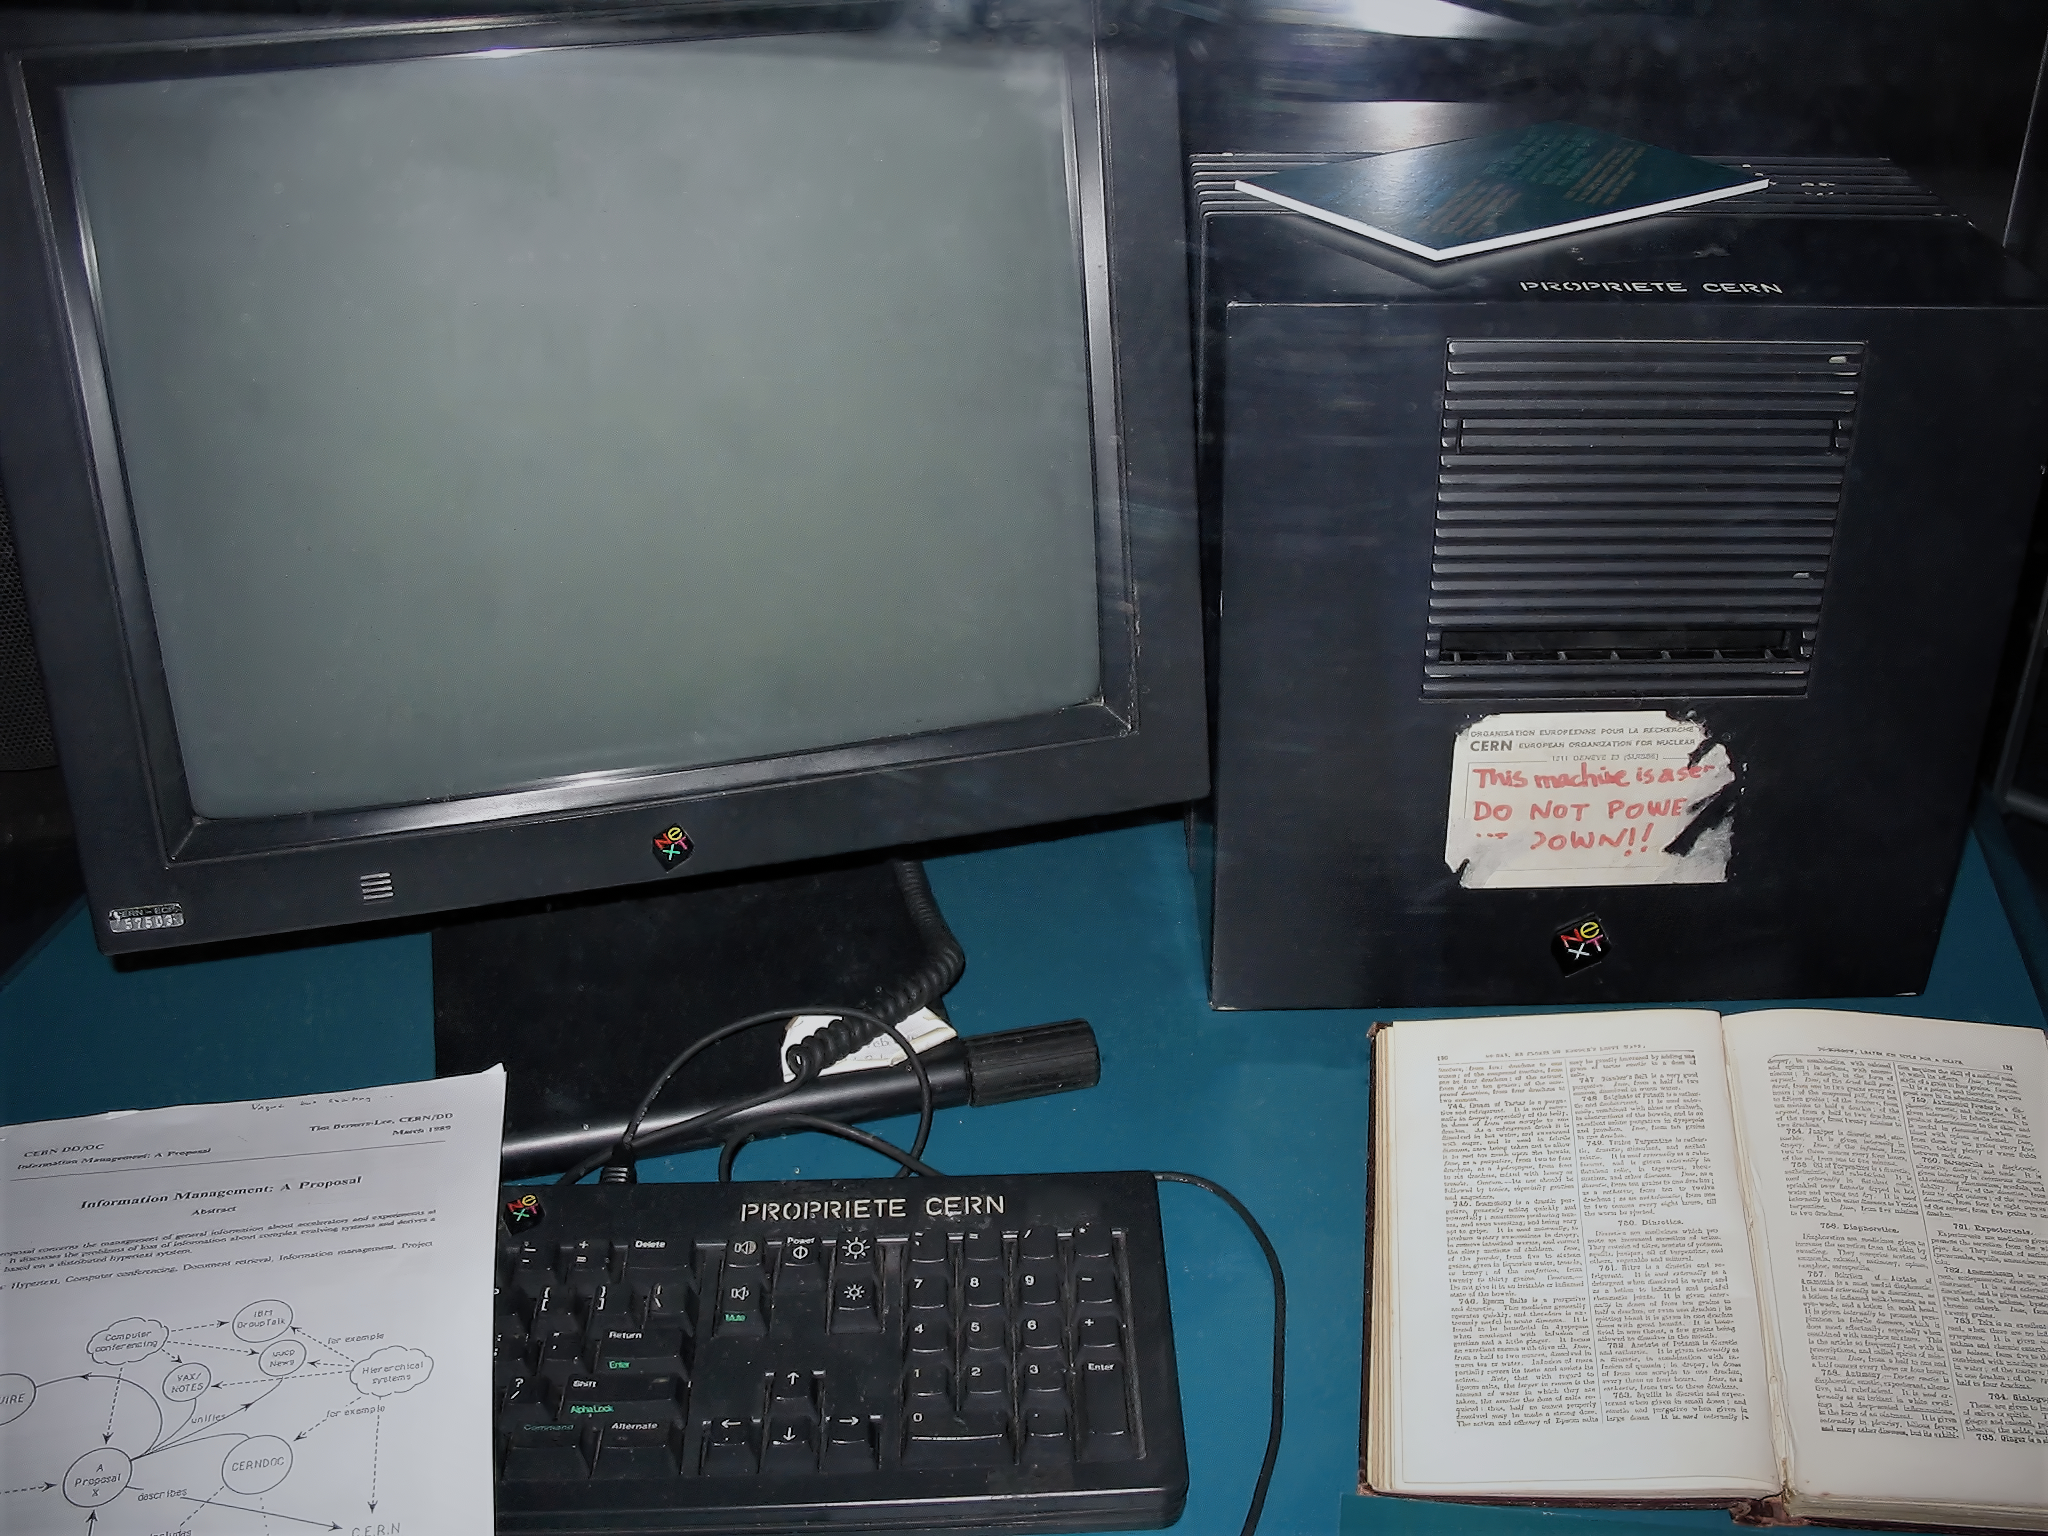
\includegraphics[width=\textwidth]{fw}
        \caption{Setup na kterém běžela první webovás tránka.}
    \end{figure}
\end{column}
\end{columns}
\end{frame}

\subsection{e-mail}
\setbeamertemplate{background}
{
    
\includegraphics[width=\paperwidth,height=\paperheight]{AICStyleData/logos/mene_polygonu_bg.png}
}
\begin{frame}{Internetové služby: e-mail}
\vspace{-0.75cm}
\begin{itemize}
    \item Používá protokol SMTP (simple mail transfer protocol), který byl založen roku 1982.
    \item E-mailový klient je program, který posílá e-maily. Ty stahuje z poštovního serveru pomocí protokolů POP nebo IMAC (Ve větších společnostech se někdy používají komerční protokoly, jako například Microsoft Exchange Server.).
\end{itemize}
\textbf{\large{Jak funguje poslání e-mailu?}}
\begin{enumerate}
    \item Odesílatel napíše e-mail. 
    \item Klient pomocí protokolu SMTP pošle zprávu softwaru MTA (mail transfer agend) (může běžet na nějakém serveru nebo přímo na počítači odesílatele).
    \item Program MTA zjistí jméno domény (část e-mailové adresy za @) v DNS (domain name system), aby zjistil mail exchange server.
    \item MTA pošle zprávu mail exchange serveru pomocí protokolu SMPT. Domény mají i záložní mail exchange servery.
    \item Mail exchange server zprávu doručí do schránky adresáta.
    \item Ze schránky adresáta poštovní klient stáhne zprávu pomocí protokolu POP nebo IMAP. 
\end{enumerate}

\end{frame}

\subsection{Volání ořes internet}
\setbeamertemplate{background}
{
    
\includegraphics[width=\paperwidth,height=\paperheight]{AICStyleData/logos/mene_polygonu_bg.png}
}
\begin{frame}{Volání pomocí internetu (VoIP)}
    \begin{itemize}
        \item Voice over Internet Protocol
        \item 
    \end{itemize}

\end{frame}


\finalpagetext{Děkuji za pozornost}
%----------------------------------------------------------------------------------------
\makefinalpage
%----------------------------------------------------------------------------------------
\end{document}
